% Options for packages loaded elsewhere
\PassOptionsToPackage{unicode}{hyperref}
\PassOptionsToPackage{hyphens}{url}
%
\documentclass[
]{article}
\usepackage{amsmath,amssymb}
\usepackage{lmodern}
\usepackage{iftex}
\ifPDFTeX
  \usepackage[T1]{fontenc}
  \usepackage[utf8]{inputenc}
  \usepackage{textcomp} % provide euro and other symbols
\else % if luatex or xetex
  \usepackage{unicode-math}
  \defaultfontfeatures{Scale=MatchLowercase}
  \defaultfontfeatures[\rmfamily]{Ligatures=TeX,Scale=1}
\fi
% Use upquote if available, for straight quotes in verbatim environments
\IfFileExists{upquote.sty}{\usepackage{upquote}}{}
\IfFileExists{microtype.sty}{% use microtype if available
  \usepackage[]{microtype}
  \UseMicrotypeSet[protrusion]{basicmath} % disable protrusion for tt fonts
}{}
\makeatletter
\@ifundefined{KOMAClassName}{% if non-KOMA class
  \IfFileExists{parskip.sty}{%
    \usepackage{parskip}
  }{% else
    \setlength{\parindent}{0pt}
    \setlength{\parskip}{6pt plus 2pt minus 1pt}}
}{% if KOMA class
  \KOMAoptions{parskip=half}}
\makeatother
\usepackage{xcolor}
\usepackage[margin=1in]{geometry}
\usepackage{graphicx}
\makeatletter
\def\maxwidth{\ifdim\Gin@nat@width>\linewidth\linewidth\else\Gin@nat@width\fi}
\def\maxheight{\ifdim\Gin@nat@height>\textheight\textheight\else\Gin@nat@height\fi}
\makeatother
% Scale images if necessary, so that they will not overflow the page
% margins by default, and it is still possible to overwrite the defaults
% using explicit options in \includegraphics[width, height, ...]{}
\setkeys{Gin}{width=\maxwidth,height=\maxheight,keepaspectratio}
% Set default figure placement to htbp
\makeatletter
\def\fps@figure{htbp}
\makeatother
\setlength{\emergencystretch}{3em} % prevent overfull lines
\providecommand{\tightlist}{%
  \setlength{\itemsep}{0pt}\setlength{\parskip}{0pt}}
\setcounter{secnumdepth}{-\maxdimen} % remove section numbering
\ifLuaTeX
  \usepackage{selnolig}  % disable illegal ligatures
\fi
\IfFileExists{bookmark.sty}{\usepackage{bookmark}}{\usepackage{hyperref}}
\IfFileExists{xurl.sty}{\usepackage{xurl}}{} % add URL line breaks if available
\urlstyle{same} % disable monospaced font for URLs
\hypersetup{
  pdftitle={Assignment 1},
  pdfauthor={Ferrara Lorenzo, Lucchini Marco},
  hidelinks,
  pdfcreator={LaTeX via pandoc}}

\title{Assignment 1}
\author{Ferrara Lorenzo, Lucchini Marco}
\date{}

\begin{document}
\maketitle

\hypertarget{description}{%
\subsection{Description}\label{description}}

\hypertarget{the-data-were-collected-during-a-study-of-the-settlement-pattern-of-common-terns-on-a-small-islet-in-the-delta-debre-hernandez-and-ruiz-range3-particularly-in-the-mouths-of-the-ebre-river.-the-islet-was-inspected-at-two-day-intervals-throughout-the-range0-breeding-season.-the-data-include-the-location-of-each-nest-its-elevation-above-sea-level-and-elevations-at-a-number-of-additional-points-points-without-nest-on-the-islet.-in-the-file-called-elevationsislet.txt-contains-the-information-of-the-coordinates-and-elevation-above-sea-and-in-file-called-poly84.txt-contains-the-coordinates-of-the-borders-of-the-islet.-the-aim-is-to-predict-the-elevation-above-sea-level-along-the-small-islet-using-a-kriging-interpolation.}{%
\subsubsection{The data were collected during a study of the settlement
pattern of common terns on a small islet in the Delta d'Ebre (Hernandez
and Ruiz, range3), particularly in the mouths of the Ebre river. The
islet was inspected at two-day intervals throughout the range0 breeding
season. The data include the location of each nest, its elevation above
sea level, and elevations at a number of additional points (points
without nest) on the islet. In the file called elevationsIslet.txt,
contains the information of the coordinates and elevation above sea, and
in file, called poly84.txt contains the coordinates of the borders of
the islet. The aim is to predict the elevation above sea level along the
small islet using a kriging
interpolation.}\label{the-data-were-collected-during-a-study-of-the-settlement-pattern-of-common-terns-on-a-small-islet-in-the-delta-debre-hernandez-and-ruiz-range3-particularly-in-the-mouths-of-the-ebre-river.-the-islet-was-inspected-at-two-day-intervals-throughout-the-range0-breeding-season.-the-data-include-the-location-of-each-nest-its-elevation-above-sea-level-and-elevations-at-a-number-of-additional-points-points-without-nest-on-the-islet.-in-the-file-called-elevationsislet.txt-contains-the-information-of-the-coordinates-and-elevation-above-sea-and-in-file-called-poly84.txt-contains-the-coordinates-of-the-borders-of-the-islet.-the-aim-is-to-predict-the-elevation-above-sea-level-along-the-small-islet-using-a-kriging-interpolation.}}

\begin{verbatim}
##             x        y data
## 1 10.39413323 70.11006   84
## 2  6.89985037 71.10941   84
## 3  1.90801770 68.11136   84
## 4 -1.08708190 61.61559   84
## 5 -2.08544844 54.62015   84
## 6 -0.08871537 45.62600   84
\end{verbatim}

\begin{verbatim}
##           x          y data
## 1  98.57754  0.8906123 17.6
## 2 113.59737 19.5085930 27.1
## 3 110.53511 39.6851815 16.4
## 4 105.27965 28.3568305 -9.5
## 5  95.20204  8.4319902  6.1
## 6 102.96788 53.0629008 -0.5
\end{verbatim}

\hypertarget{explore-the-requirement-of-stationary-mean-of-the-process.-in-case-this-requirement-is-not-met-detrend-the-data-to-ensure-that-the-process-is-stationary-in-mean.-discuss-the-results-and-show-the-plot-of-the-results}{%
\subsubsection{1) Explore the requirement of stationary mean of the
process. In case this requirement is not met, detrend the data to ensure
that the process is stationary in mean. Discuss the results and show the
plot of the
results}\label{explore-the-requirement-of-stationary-mean-of-the-process.-in-case-this-requirement-is-not-met-detrend-the-data-to-ensure-that-the-process-is-stationary-in-mean.-discuss-the-results-and-show-the-plot-of-the-results}}

Firstly, we plot the locations to see the spatial distribution of the
data

\includegraphics{Assignment_1_files/figure-latex/unnamed-chunk-5-1.pdf}

METTERLO IN SCALA D COLORI

We also look at the distribution in relation to the x-coordinates (E-W)
and y-coordinates(N-S).

\includegraphics{Assignment_1_files/figure-latex/unnamed-chunk-6-1.pdf}

\includegraphics{Assignment_1_files/figure-latex/unnamed-chunk-7-1.pdf}

The plots show a concentration of high values in the east (data are
centered in x=50) and in the north (data are very dense from y=0 to
y=50)

The process doesn't seem stationary, indeed there is a clear quadratic
trend along the x direction. In addition we try using the y direction as
regressor, to find a possible linear or quadratic trend.

\begin{verbatim}
## 
## Call:
## lm(formula = data ~ x + y + I(x^2) + I(y^2), data = dataset)
## 
## Residuals:
##     Min      1Q  Median      3Q     Max 
## -22.639  -6.417  -0.964   6.024  22.744 
## 
## Coefficients:
##               Estimate Std. Error t value Pr(>|t|)    
## (Intercept) 17.4502678  2.8429177   6.138 7.78e-09 ***
## x           -0.4938096  0.1103379  -4.475 1.55e-05 ***
## y            0.0349038  0.0570014   0.612    0.541    
## I(x^2)       0.0040706  0.0009267   4.393 2.17e-05 ***
## I(y^2)       0.0019508  0.0008841   2.206    0.029 *  
## ---
## Signif. codes:  0 '***' 0.001 '**' 0.01 '*' 0.05 '.' 0.1 ' ' 1
## 
## Residual standard error: 10.19 on 143 degrees of freedom
## Multiple R-squared:  0.2026, Adjusted R-squared:  0.1803 
## F-statistic: 9.082 on 4 and 143 DF,  p-value: 1.446e-06
\end{verbatim}

The linear term in y doesn't seem significant, so we remove it.

\begin{verbatim}
## 
## Call:
## lm(formula = data ~ x + I(x^2) + I(y^2), data = dataset)
## 
## Residuals:
##     Min      1Q  Median      3Q     Max 
## -22.768  -6.656  -1.081   6.166  22.879 
## 
## Coefficients:
##               Estimate Std. Error t value Pr(>|t|)    
## (Intercept) 18.3842839  2.3938539   7.680 2.23e-12 ***
## x           -0.5192823  0.1019735  -5.092 1.09e-06 ***
## I(x^2)       0.0042621  0.0008705   4.896 2.59e-06 ***
## I(y^2)       0.0023697  0.0005587   4.241 3.96e-05 ***
## ---
## Signif. codes:  0 '***' 0.001 '**' 0.01 '*' 0.05 '.' 0.1 ' ' 1
## 
## Residual standard error: 10.17 on 144 degrees of freedom
## Multiple R-squared:  0.2005, Adjusted R-squared:  0.1838 
## F-statistic: 12.04 on 3 and 144 DF,  p-value: 4.456e-07
\end{verbatim}

Now we have obtained a model in which all regressor seem to be
significant =\textgreater{} So we save the residuals of our linear model
and look at the de-trended data:

\begin{verbatim}
##           x          y data residuals
## 1  98.57754  0.8906123 17.6     8.987
## 2 113.59737 19.5085930 27.1    11.804
## 3 110.53511 39.6851815 16.4    -0.391
## 4 105.27965 28.3568305 -9.5   -22.360
## 5  95.20204  8.4319902  6.1    -1.645
## 6 102.96788 53.0629008 -0.5   -17.275
\end{verbatim}

\includegraphics{Assignment_1_files/figure-latex/unnamed-chunk-10-1.pdf}

\includegraphics{Assignment_1_files/figure-latex/unnamed-chunk-11-1.pdf}

We don't notice any particular trend so this new dataset seems
stationary! And now the data seems distributed around 0.

\hypertarget{explore-the-spatial-dependence-of-the-elevation-variable-using-the-variogram-cloud-and-bins-and-the-empirical-variogram.-discuss-the-results-and-plot-them}{%
\subsubsection{2) Explore the spatial dependence of the elevation
variable using the variogram cloud and bins and the empirical variogram.
Discuss the results and plot
them}\label{explore-the-spatial-dependence-of-the-elevation-variable-using-the-variogram-cloud-and-bins-and-the-empirical-variogram.-discuss-the-results-and-plot-them}}

\hypertarget{variogram-could}{%
\subsubsection{Variogram Could}\label{variogram-could}}

\begin{verbatim}
## variog: computing omnidirectional variogram
\end{verbatim}

\includegraphics{Assignment_1_files/figure-latex/unnamed-chunk-12-1.pdf}

The variability at small distances appears a bit greater than that for
larger distances. =\textgreater{} We reduce the density of the plot by
reducing the maximum distance over which the variance are calculate.

\begin{verbatim}
## variog: computing omnidirectional variogram
\end{verbatim}

\includegraphics{Assignment_1_files/figure-latex/unnamed-chunk-13-1.pdf}

\begin{verbatim}
## variog: computing omnidirectional variogram
\end{verbatim}

\includegraphics{Assignment_1_files/figure-latex/unnamed-chunk-14-1.pdf}

\begin{verbatim}
##  [1] TRUE TRUE TRUE TRUE TRUE TRUE TRUE TRUE TRUE TRUE TRUE TRUE TRUE
\end{verbatim}

=\textgreater{} All the bins have at least pairs.min=30 observations
each, indeed they have:

\begin{verbatim}
##  [1]  764 1158 1112  829  742  751  719  615  652  903 1040  982  427
\end{verbatim}

Empirical Variogram

\begin{verbatim}
## variog: computing omnidirectional variogram
\end{verbatim}

\includegraphics{Assignment_1_files/figure-latex/unnamed-chunk-18-1.pdf}

\begin{verbatim}
## variog: computing omnidirectional variogram
\end{verbatim}

\includegraphics{Assignment_1_files/figure-latex/unnamed-chunk-19-1.pdf}

In the variogram of the residuals the values increases until certain
distance, and then they keep constant.

\hypertarget{check-the-hypothesis-of-the-spatial-independence}{%
\subsubsection{3) Check the hypothesis of the spatial
independence}\label{check-the-hypothesis-of-the-spatial-independence}}

To check the hypothesis of the spatial independence we use a Monte Carlo
approach

\begin{verbatim}
## variog.env: generating 1000 simulations by permutating data values
## variog.env: computing the empirical variogram for the 1000 simulations
## variog.env: computing the envelops
\end{verbatim}

\includegraphics{Assignment_1_files/figure-latex/unnamed-chunk-20-1.pdf}

All the values of the empirical variogram are inside the envelope,
therefore the process has no spatial dependence.

\hypertarget{check-the-isotropy-property-of-the-process.-comment-the-results-its-not-necessary-to-overcome-the-anisotropy.}{%
\subsubsection{4) Check the isotropy property of the process. Comment
the results, it's not necessary to overcome the
anisotropy.}\label{check-the-isotropy-property-of-the-process.-comment-the-results-its-not-necessary-to-overcome-the-anisotropy.}}

To check the anisotropy we need to compute the directional variogram in
the 4 main directions: 0º, 45º,90º and 135º.

\begin{verbatim}
## variog: computing variogram for direction = 0 degrees (0 radians)
##         tolerance angle = 22.5 degrees (0.393 radians)
## variog: computing variogram for direction = 45 degrees (0.785 radians)
##         tolerance angle = 22.5 degrees (0.393 radians)
## variog: computing variogram for direction = 90 degrees (1.571 radians)
##         tolerance angle = 22.5 degrees (0.393 radians)
## variog: computing variogram for direction = 135 degrees (2.356 radians)
##         tolerance angle = 22.5 degrees (0.393 radians)
## variog: computing omnidirectional variogram
\end{verbatim}

\includegraphics{Assignment_1_files/figure-latex/unnamed-chunk-21-1.pdf}

\begin{verbatim}
## variog: computing variogram for direction = 0 degrees (0 radians)
##         tolerance angle = 22.5 degrees (0.393 radians)
## variog: computing variogram for direction = 45 degrees (0.785 radians)
##         tolerance angle = 22.5 degrees (0.393 radians)
## variog: computing variogram for direction = 90 degrees (1.571 radians)
##         tolerance angle = 22.5 degrees (0.393 radians)
## variog: computing variogram for direction = 135 degrees (2.356 radians)
##         tolerance angle = 22.5 degrees (0.393 radians)
## variog: computing omnidirectional variogram
\end{verbatim}

\includegraphics{Assignment_1_files/figure-latex/unnamed-chunk-22-1.pdf}

The directional variograms don't seem to be perfectly overlapping: they
might have the same range, but not the same sill.

Let's also observe the Rose Diagram:

\hypertarget{credo}{%
\section{credo?}\label{credo}}

\begin{verbatim}
## variog: computing variogram for direction = 45 degrees (0.785 radians)
##         tolerance angle = 45 degrees (0.785 radians)
## variog: computing variogram for direction = 90 degrees (1.571 radians)
##         tolerance angle = 45 degrees (0.785 radians)
## variog: computing variogram for direction = 135 degrees (2.356 radians)
##         tolerance angle = 45 degrees (0.785 radians)
## variog: computing variogram for direction = 180 degrees (3.142 radians)
##         tolerance angle = 45 degrees (0.785 radians)
\end{verbatim}

\includegraphics{Assignment_1_files/figure-latex/unnamed-chunk-23-1.pdf}

We can observe that the Rose diagram is more or less a circle. At
different directions, the variance is reached more or less at the same
range. Then, this process is isotropic.

OPPURE

We notice that the Rose diagram is not circular, but it is rather
elliptical, with major range in the 90 direction =\textgreater{} Then we
can't make the assumption of isotropic process.

MAGARI è IL CASO DI FARE IL CLOUD CON LA ROBUST WAY?

\begin{verbatim}
## variog: computing omnidirectional variogram
\end{verbatim}

\begin{verbatim}
## variog: computing omnidirectional variogram
\end{verbatim}

\begin{verbatim}
## variog: computing omnidirectional variogram
\end{verbatim}

\includegraphics{Assignment_1_files/figure-latex/unnamed-chunk-24-1.pdf}

\hypertarget{propose-four-theoretical-variogram-and-estimate-the-parameters-via-restricted-maximum-likelihood-or-weighed-least-square.-select-the-two-variograms-which-best-fit-the-data.-explain-the-parameters-of-the-chosen-variogram-sill-nugget-range-and-kappa.}{%
\subsubsection{5) Propose four theoretical variogram and estimate the
parameters via restricted maximum likelihood or weighed least square.
Select the two variograms which best fit the data. Explain the
parameters of the chosen variogram (sill, nugget, range and
kappa).}\label{propose-four-theoretical-variogram-and-estimate-the-parameters-via-restricted-maximum-likelihood-or-weighed-least-square.-select-the-two-variograms-which-best-fit-the-data.-explain-the-parameters-of-the-chosen-variogram-sill-nugget-range-and-kappa.}}

\begin{verbatim}
## variog: computing omnidirectional variogram
\end{verbatim}

\includegraphics{Assignment_1_files/figure-latex/unnamed-chunk-25-1.pdf}

ho messo gli stessi dati iniziali per goni fitting, dovrei cercare
quelli azzeccati con eyefit per ognuna?

\hypertarget{exponential}{%
\paragraph{Exponential}\label{exponential}}

\begin{verbatim}
## variofit: model parameters estimated by WLS (weighted least squares):
## covariance model is: exponential
## parameter estimates:
##   tausq sigmasq     phi 
## 22.3110 83.9476  0.0000 
## Practical Range with cor=0.05 for asymptotic range: 0.0001159668
## 
## variofit: minimised weighted sum of squares = 236.0217
\end{verbatim}

\hypertarget{gaussian}{%
\paragraph{Gaussian}\label{gaussian}}

\begin{verbatim}
## variofit: model parameters estimated by WLS (weighted least squares):
## covariance model is: gaussian
## parameter estimates:
##   tausq sigmasq     phi 
## 20.5249 85.7337  0.0000 
## Practical Range with cor=0.05 for asymptotic range: 0.0001159668
## 
## variofit: minimised weighted sum of squares = 236.0217
\end{verbatim}

\hypertarget{spherical}{%
\paragraph{Spherical}\label{spherical}}

\begin{verbatim}
## variofit: model parameters estimated by WLS (weighted least squares):
## covariance model is: spherical
## parameter estimates:
##   tausq sigmasq     phi 
## 34.9006 71.3580  0.0000 
## Practical Range with cor=0.05 for asymptotic range: 0
## 
## variofit: minimised weighted sum of squares = 236.0217
\end{verbatim}

\hypertarget{matern}{%
\paragraph{Matern}\label{matern}}

\begin{verbatim}
## variofit: model parameters estimated by WLS (weighted least squares):
## covariance model is: matern
## parameter estimates:
##   tausq sigmasq     phi   kappa 
## 25.0162 81.2424  0.0000  1.0000 
## Practical Range with cor=0.05 for asymptotic range: 0.0001159668
## 
## variofit: minimised weighted sum of squares = 236.0217
\end{verbatim}

\hypertarget{computing-envelops-for-empirical-variograms.}{%
\paragraph{Computing envelops for empirical
variograms.}\label{computing-envelops-for-empirical-variograms.}}

\includegraphics{Assignment_1_files/figure-latex/unnamed-chunk-33-1.pdf}

\hypertarget{lets-compare-the-different-models}{%
\paragraph{Let's compare the different
models}\label{lets-compare-the-different-models}}

\begin{verbatim}
##         model sum.of.squares
## 1 exponential       236.0217
## 2    gaussian       236.0217
## 3   spherical       236.0217
## 4      matern       236.0217
\end{verbatim}

\hypertarget{exponential-1}{%
\paragraph{Exponential}\label{exponential-1}}

\begin{verbatim}
## likfit: estimated model parameters:
##     beta    tausq  sigmasq      phi 
## "-2.585" "34.233" "69.359" " 5.665" 
## Practical Range with cor=0.05 for asymptotic range: 16.96957
## 
## likfit: maximised log-likelihood = -535.2
\end{verbatim}

\hypertarget{gaussian-1}{%
\paragraph{Gaussian}\label{gaussian-1}}

\begin{verbatim}
## likfit: estimated model parameters:
##     beta    tausq  sigmasq      phi 
## "-2.742" "40.939" "65.117" " 5.476" 
## Practical Range with cor=0.05 for asymptotic range: 9.478475
## 
## likfit: maximised log-likelihood = -533.5
\end{verbatim}

\hypertarget{spherical-1}{%
\paragraph{Spherical}\label{spherical-1}}

\begin{verbatim}
## likfit: estimated model parameters:
##     beta    tausq  sigmasq      phi 
## "-2.731" "36.356" "67.835" "12.770" 
## Practical Range with cor=0.05 for asymptotic range: 12.77019
## 
## likfit: maximised log-likelihood = -534
\end{verbatim}

NON CAPISCO QUALE SIA LA DIFFERENZA? KAPPA COS'è?

\begin{verbatim}
## ---------------------------------------------------------------
## likfit: likelihood maximisation using the function optim.
## likfit: Use control() to pass additional
##          arguments for the maximisation function.
##         For further details see documentation for optim.
## likfit: It is highly advisable to run this function several
##         times with different initial values for the parameters.
## likfit: WARNING: This step can be time demanding!
## ---------------------------------------------------------------
## likfit: end of numerical maximisation.
\end{verbatim}

\begin{verbatim}
## likfit: estimated model parameters:
##      beta     tausq   sigmasq       phi     kappa 
## "-2.7383" "40.8641" "65.1187" " 0.3673" "55.9395" 
## Practical Range with cor=0.05 for asymptotic range: 9.55232
## 
## likfit: maximised log-likelihood = -533.5
\end{verbatim}

\begin{verbatim}
## ---------------------------------------------------------------
## likfit: likelihood maximisation using the function optim.
## likfit: Use control() to pass additional
##          arguments for the maximisation function.
##         For further details see documentation for optim.
## likfit: It is highly advisable to run this function several
##         times with different initial values for the parameters.
## likfit: WARNING: This step can be time demanding!
## ---------------------------------------------------------------
## likfit: end of numerical maximisation.
\end{verbatim}

\begin{verbatim}
## likfit: estimated model parameters:
##     beta    tausq  sigmasq      phi 
## "-2.585" "34.233" "69.359" " 5.665" 
## Practical Range with cor=0.05 for asymptotic range: 16.96959
## 
## likfit: maximised log-likelihood = -535.2
\end{verbatim}

\includegraphics{Assignment_1_files/figure-latex/unnamed-chunk-40-1.pdf}

\includegraphics{Assignment_1_files/figure-latex/unnamed-chunk-42-1.pdf}

Let's compare the different models

\begin{verbatim}
##         model loglikelihood
## 1 exponential     -535.2439
## 2    gaussian     -533.4938
## 3   spherical     -533.9930
## 4      matern     -535.2439
\end{verbatim}

\hypertarget{predict-the-elevations-along-all-the-area-of-study-using-the-two-variogram-selected-in-point-4.-discuss-the-type-of-kriging-chosen}{%
\subsubsection{6) Predict the elevations along all the area of study
using the two variogram selected in point 4. Discuss the type of kriging
chosen:}\label{predict-the-elevations-along-all-the-area-of-study-using-the-two-variogram-selected-in-point-4.-discuss-the-type-of-kriging-chosen}}

\hypertarget{a.-compare-both-kriging-predictions-using-cross-validation-and-propose-the-best-model.}{%
\subsubsection{a. Compare both kriging predictions using
cross-validation, and propose the best
model.}\label{a.-compare-both-kriging-predictions-using-cross-validation-and-propose-the-best-model.}}

\hypertarget{b.-show-the-predictions-and-their-standard-errors.}{%
\subsubsection{b. Show the predictions and their standard
errors.}\label{b.-show-the-predictions-and-their-standard-errors.}}

\includegraphics{Assignment_1_files/figure-latex/unnamed-chunk-44-1.pdf}

\hypertarget{gaussian-2}{%
\paragraph{Gaussian}\label{gaussian-2}}

\begin{verbatim}
## krige.conv: model with constant mean
## krige.conv: Kriging performed using global neighbourhood
\end{verbatim}

\includegraphics{Assignment_1_files/figure-latex/unnamed-chunk-45-1.pdf}

\includegraphics{Assignment_1_files/figure-latex/unnamed-chunk-46-1.pdf}

\includegraphics{Assignment_1_files/figure-latex/unnamed-chunk-47-1.pdf}

\begin{verbatim}
## xvalid: number of data locations       = 148
## xvalid: number of validation locations = 148
## xvalid: performing cross-validation at location ... 1, 2, 3, 4, 5, 6, 7, 8, 9, 10, 11, 12, 13, 14, 15, 16, 17, 18, 19, 20, 21, 22, 23, 24, 25, 26, 27, 28, 29, 30, 31, 32, 33, 34, 35, 36, 37, 38, 39, 40, 41, 42, 43, 44, 45, 46, 47, 48, 49, 50, 51, 52, 53, 54, 55, 56, 57, 58, 59, 60, 61, 62, 63, 64, 65, 66, 67, 68, 69, 70, 71, 72, 73, 74, 75, 76, 77, 78, 79, 80, 81, 82, 83, 84, 85, 86, 87, 88, 89, 90, 91, 92, 93, 94, 95, 96, 97, 98, 99, 100, 101, 102, 103, 104, 105, 106, 107, 108, 109, 110, 111, 112, 113, 114, 115, 116, 117, 118, 119, 120, 121, 122, 123, 124, 125, 126, 127, 128, 129, 130, 131, 132, 133, 134, 135, 136, 137, 138, 139, 140, 141, 142, 143, 144, 145, 146, 147, 148, 
## xvalid: end of cross-validation
\end{verbatim}

\begin{verbatim}
## [1] "data"      "predicted" "krige.var" "error"     "std.error" "prob"
\end{verbatim}

\begin{verbatim}
##   index     value
## 1   VC1 0.0389848
## 2   VC2 1.0370798
## 3   VC3 8.7075045
\end{verbatim}

\hypertarget{spherical-2}{%
\paragraph{Spherical}\label{spherical-2}}

\begin{verbatim}
## krige.conv: model with constant mean
## krige.conv: Kriging performed using global neighbourhood
\end{verbatim}

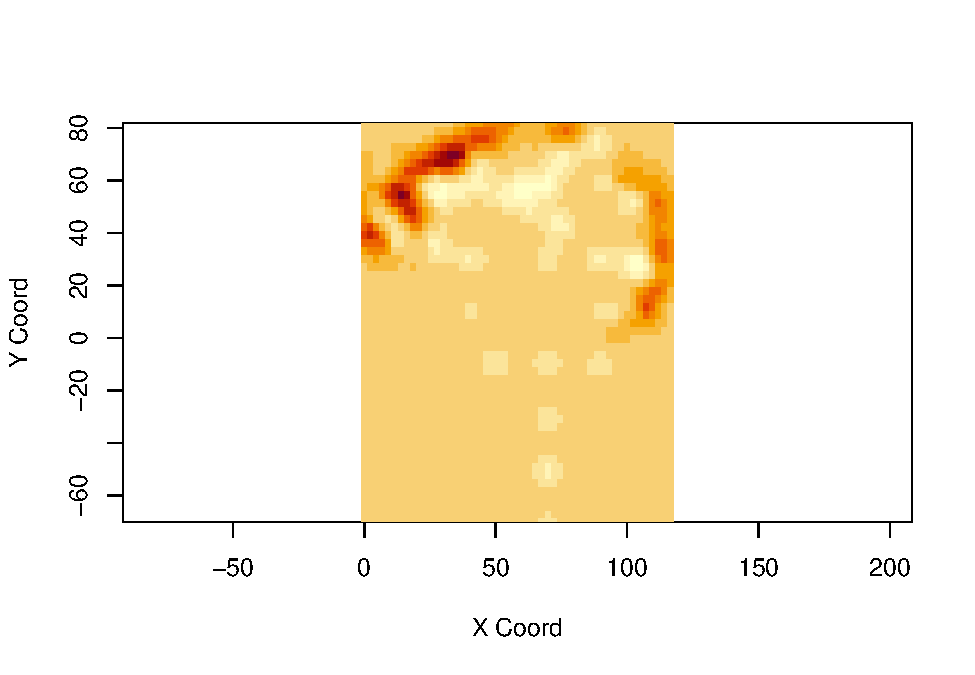
\includegraphics{Assignment_1_files/figure-latex/unnamed-chunk-50-1.pdf}

\includegraphics{Assignment_1_files/figure-latex/unnamed-chunk-51-1.pdf}

\includegraphics{Assignment_1_files/figure-latex/unnamed-chunk-52-1.pdf}

\begin{verbatim}
## xvalid: number of data locations       = 148
## xvalid: number of validation locations = 148
## xvalid: performing cross-validation at location ... 1, 2, 3, 4, 5, 6, 7, 8, 9, 10, 11, 12, 13, 14, 15, 16, 17, 18, 19, 20, 21, 22, 23, 24, 25, 26, 27, 28, 29, 30, 31, 32, 33, 34, 35, 36, 37, 38, 39, 40, 41, 42, 43, 44, 45, 46, 47, 48, 49, 50, 51, 52, 53, 54, 55, 56, 57, 58, 59, 60, 61, 62, 63, 64, 65, 66, 67, 68, 69, 70, 71, 72, 73, 74, 75, 76, 77, 78, 79, 80, 81, 82, 83, 84, 85, 86, 87, 88, 89, 90, 91, 92, 93, 94, 95, 96, 97, 98, 99, 100, 101, 102, 103, 104, 105, 106, 107, 108, 109, 110, 111, 112, 113, 114, 115, 116, 117, 118, 119, 120, 121, 122, 123, 124, 125, 126, 127, 128, 129, 130, 131, 132, 133, 134, 135, 136, 137, 138, 139, 140, 141, 142, 143, 144, 145, 146, 147, 148, 
## xvalid: end of cross-validation
\end{verbatim}

\begin{verbatim}
##   index      value
## 1   VC1 0.03374952
## 2   VC2 1.03287030
## 3   VC3 8.73934527
\end{verbatim}

\hypertarget{exponential-2}{%
\paragraph{Exponential}\label{exponential-2}}

\begin{verbatim}
## krige.conv: model with constant mean
## krige.conv: Kriging performed using global neighbourhood
\end{verbatim}

\includegraphics{Assignment_1_files/figure-latex/unnamed-chunk-55-1.pdf}

\includegraphics{Assignment_1_files/figure-latex/unnamed-chunk-56-1.pdf}

\includegraphics{Assignment_1_files/figure-latex/unnamed-chunk-57-1.pdf}

\begin{verbatim}
## xvalid: number of data locations       = 148
## xvalid: number of validation locations = 148
## xvalid: performing cross-validation at location ... 1, 2, 3, 4, 5, 6, 7, 8, 9, 10, 11, 12, 13, 14, 15, 16, 17, 18, 19, 20, 21, 22, 23, 24, 25, 26, 27, 28, 29, 30, 31, 32, 33, 34, 35, 36, 37, 38, 39, 40, 41, 42, 43, 44, 45, 46, 47, 48, 49, 50, 51, 52, 53, 54, 55, 56, 57, 58, 59, 60, 61, 62, 63, 64, 65, 66, 67, 68, 69, 70, 71, 72, 73, 74, 75, 76, 77, 78, 79, 80, 81, 82, 83, 84, 85, 86, 87, 88, 89, 90, 91, 92, 93, 94, 95, 96, 97, 98, 99, 100, 101, 102, 103, 104, 105, 106, 107, 108, 109, 110, 111, 112, 113, 114, 115, 116, 117, 118, 119, 120, 121, 122, 123, 124, 125, 126, 127, 128, 129, 130, 131, 132, 133, 134, 135, 136, 137, 138, 139, 140, 141, 142, 143, 144, 145, 146, 147, 148, 
## xvalid: end of cross-validation
\end{verbatim}

\begin{verbatim}
##   index      value
## 1   VC1 0.02709577
## 2   VC2 1.02576588
## 3   VC3 8.75339750
\end{verbatim}

\hypertarget{matern-1}{%
\paragraph{Matern}\label{matern-1}}

\begin{verbatim}
## krige.conv: model with constant mean
## krige.conv: Kriging performed using global neighbourhood
\end{verbatim}

\includegraphics{Assignment_1_files/figure-latex/unnamed-chunk-60-1.pdf}

\includegraphics{Assignment_1_files/figure-latex/unnamed-chunk-61-1.pdf}

\includegraphics{Assignment_1_files/figure-latex/unnamed-chunk-62-1.pdf}

\begin{verbatim}
## xvalid: number of data locations       = 148
## xvalid: number of validation locations = 148
## xvalid: performing cross-validation at location ... 1, 2, 3, 4, 5, 6, 7, 8, 9, 10, 11, 12, 13, 14, 15, 16, 17, 18, 19, 20, 21, 22, 23, 24, 25, 26, 27, 28, 29, 30, 31, 32, 33, 34, 35, 36, 37, 38, 39, 40, 41, 42, 43, 44, 45, 46, 47, 48, 49, 50, 51, 52, 53, 54, 55, 56, 57, 58, 59, 60, 61, 62, 63, 64, 65, 66, 67, 68, 69, 70, 71, 72, 73, 74, 75, 76, 77, 78, 79, 80, 81, 82, 83, 84, 85, 86, 87, 88, 89, 90, 91, 92, 93, 94, 95, 96, 97, 98, 99, 100, 101, 102, 103, 104, 105, 106, 107, 108, 109, 110, 111, 112, 113, 114, 115, 116, 117, 118, 119, 120, 121, 122, 123, 124, 125, 126, 127, 128, 129, 130, 131, 132, 133, 134, 135, 136, 137, 138, 139, 140, 141, 142, 143, 144, 145, 146, 147, 148, 
## xvalid: end of cross-validation
\end{verbatim}

\begin{verbatim}
##   index      value
## 1   VC1 0.02709578
## 2   VC2 1.02576586
## 3   VC3 8.75339659
\end{verbatim}

\end{document}
